\section{Introducción}

Desde el trabajo pionero de Song\cite{Song2005} se ha considerado que las redes complejas consisten en patrones auto-similares bajo transformaciones de escala. Se han proporcionado diferentes estrategias basadas en la cobertura de cajas para caracterizar la dimensión fractal en redes complejas. Sin embargo, la dimensión fractal no es suficiente para caracterizar las propiedades fractales de las redes complejas, por esta razón para el análisis multifractal se propone calcular la dimensión fractal a medida que se realiza un escalado de la red.

El análisis multifractal es útil para caracterizar la heterogeneidad espacial de las redes complejas, ya que considera que no sólo existe un patrón de estructuras dentro de las redes complejas.

Las diferentes estrategias permiten calcular los exponentes de masa $\tau_q$, que representan como cambia la densidad de la red a medida que se escala por un factor real $q$ y la pendiente de esta recta para un $q$ dado viene siendo la dimensión fractal $D_q$, de esta forma se puede estudiar los cambios en la estructura de la red a medida que esta es escalada.

Si la función $D_q$ es una linea recta, se dice que la red es monofractal, en caso contrario, es multifractal. Esta función tiene algunos valores clave\cite{Halsey1986}: $D_0$ es la dimensión fractal, $D_1$ es la dimensión  informacional y $D_2$ es la correlación.

\section{Estrategias de cubrimiento de cajas}

Este método es una herramienta para estimar la dimensión fractal de objetos en un espacio Euclidiano. Sin embargo, la métrica no es relevante para redes complejas, por es razón se considera la longitud del camino más corto entre un par de nodos como métrica. 

Para una red cualquiera, se toma $N_B$ como el número de cajas de radio $r_B$ que se necesitan para cubrir toda la red, por lo tanto la dimensión fractal $d_B$ se caracteriza de la siguiente forma:

\begin{equation}
    N_B \approx r_B^{d_B}
\end{equation}

El algoritmo más común para obtener esta medida es:

\begin{enumerate}
    \item Seleccione un nodo aleatoriamente como el centro de una caja
    \item Busque los nodos a un radio $r_B$ y que no han sido cubiertos por otra caja y asígnelos a la caja
    \item Repita los pasos 1 y 2 hasta asignar los nodos a sus respectivas cajas
\end{enumerate}

La dimensión fractal con la pendiente de la regresión lineal entre $log(N_B))$ y $log(d_B)$

De este algoritmo se tienen varias variante que dependen como se seleccionan los centros:

\begin{enumerate}
    \item Selección aleatoria\cite{Kim2007B}: Seleccionando los centro de tal forma se obtenga el mínimo número de cajas.
    \item Estrategia voraz\cite{Song2007}: Seleccionando los centro de acuerdo a un problema análogo de coloreo de grados
    \item Estrategia quemada\cite{Song2007}: Consiste en permitir solapamientos entre las cajas  y cubrir la red con estas.
\end{enumerate}

Los autores de estas estrategias mediante pruebas en algunas redes, han encontrado que se obtiene una medida de dimensión fractal similar a la calculada analíticamente.



\subsubsection{Box Covering Fixed Size}

Uno de los algoritmos que se se ha propuesto, es el de \textit{Box Covering Fixed Size}\cite{Halsey1986}\cite{RendondelaTorre2017}\cite{Yu2003}, el cual consiste en considerar para una medida dada, se considera la siguiente relación:

\begin{equation}
    Z_e(q) =  \sum \limits_{\mu(B) \neq 0} \mu(B)^q
\end{equation}

Donde $q\in R$ y la suma representa todas las diferentes cajas $B$ no vacías, para un tamaño $e$ definido y que cubren toda la red. Los exponentes de masa $\tau(q)$ están definidos por:

\begin{equation}
    \tau(q) = \lim_{x \to \infty} \frac{\ln Z_e(q)}{\ln e}
\end{equation}

Las dimensiones fractales generalizadas están definidas por:

\begin{equation}
    D_q = \frac{\tau(q)}{q-1}, q \neq 1
\end{equation}

Y

\begin{equation}
    D_1 = \lim_{x \to 0} \frac{Z_{1,e}}{ln e}
\end{equation}

Donde $Z_{1,e} = \sum \limits_{\mu(B) \neq 0} \mu(B) \ln \mu(B)$

Los exponentes de masa se pueden obtener a través de una regresión lineal entre $ln(Z_e(q)$ y $ln e$, así mismo las dimensiones fractales 

Debido a que la elección de los centros de las cajas es aleatorio, esto puede afectar la medida. Si se seleccionados vértices con un gran grado (hub) se puede cubrir la red de forma eficiente, pero si son seleccionados nodos con grado bajo, pocos nodos pueden ser cubiertos. Para enfrentar este problema se propone seleccionar un conjunto T de permutaciones distintas de nodos y tomar un promedio. La sección de T, debe estar acorde al número de nodos.

El procedimiento para calcular las dimensiones fractales es:

\begin{enumerate}
    \item Se generan matrices de adyacencia y distancias
    \item En primer lugar, asegurarse que todos los nodos en la red no esté cubiertos por alguna caja
     \item Se generan T permutaciones de vértices (con todos los existentes en la red), los cuales serán seleccionado como centros de cajas en el orden de aparición
     \item Se selecciona el tamaño de una caja $r\in[1,d]$  donde $d$ es el diámetro de la red.
     \item Se selecciona el centro de la caja y se incluyen todos los nodos que están dentro de una distancia $r$ y no han sido cubiertos
     \item Se repite este proceso hasta que todos los vértices han sido cubiertos
     \item Se toma como medida $\mu(B)=\frac{N_B}{N}$ donde $N_B$ es el número de vértices en la red y $N$ es el número total de vértices.
     \item Se calcula la suma $ Z_r(q) =  \sum \limits_{\mu(B) \neq 0} \mu(B)^q$
     \item Se repiten los pasos 3-8 con cada uno de los conjuntos $T$. Se toman los promedios de $\overline{Z_r(q)} = \sum^t (Z_r(q))/T$  
\end{enumerate}

Posteriormente se realiza una regresión lineal entre $\ln \overline{Z_r(q)}$ y $\ln\frac{r}{d}$. Se debe considera el caso especial cuando $q=1$.

El algoritmo es implementado en lenguaje Python y es aplicado en las siguientes redes del Anexo A en la página \pageref{AnexoA},

Para la red libre de escala de 4000 nodos se obtiene, la relación entre $q$ y $\ln Zr$

\begin{figure}[H]
    \centering
    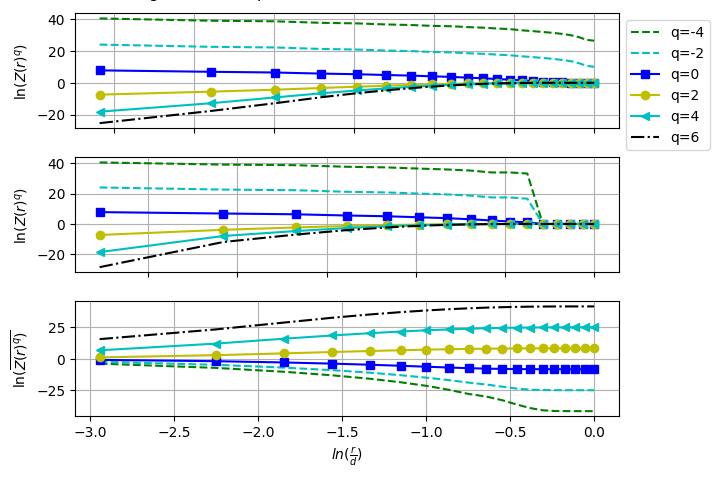
\includegraphics[scale=0.7]{Capitulo4Multifractalidad/imagenes/scaleFree4000_TqLnrBCscaleFree4000Nodes.png}
    \caption{Regresión linea para red libre de escala 4000 nodos}
\end{figure}

Cada valor de $q$ tiene su función de la cual se obtiene su pendiente, la cual corresponde a sus exponentes de masa.

\begin{figure}[H]
    \centering
    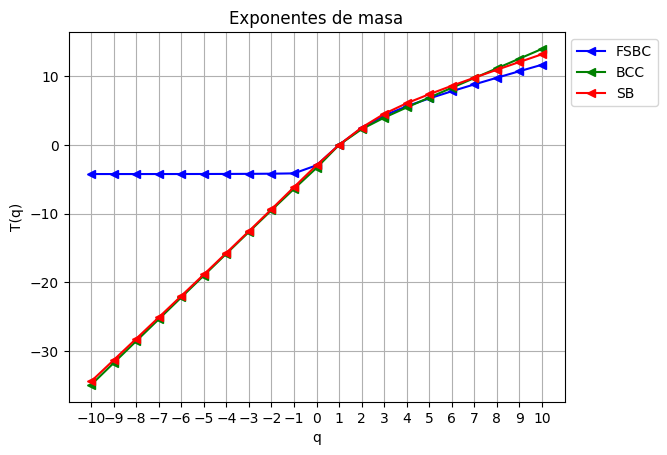
\includegraphics[scale=0.7]{Capitulo4Multifractalidad/imagenes/scaleFree4000_TqscaleFree4000Nodes.png}
    \caption{Exponentes de masa para red libre de escala 4000 nodos}
\end{figure}

Posteriormente, se realiza la transformación para obtener la dimensión fractal generalizada tomando en cuenta el caso especial para $q=1$. Es de anotar que en la práctica la dimensión se analiza para $q\geq0$

\begin{figure}[H]
    \centering
    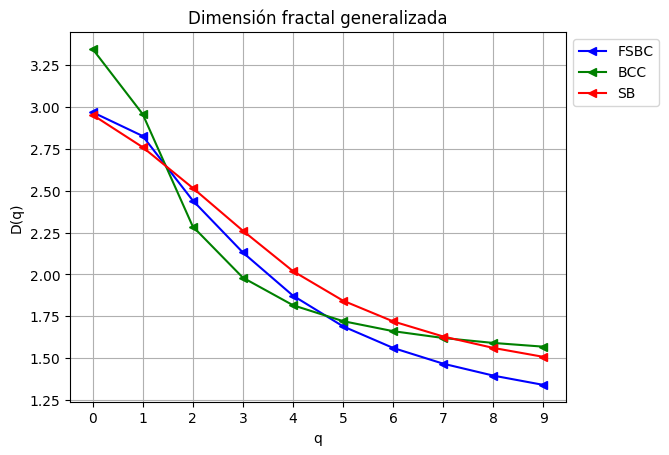
\includegraphics[scale=0.7]{Capitulo4Multifractalidad/imagenes/scaleFree4000_DqscaleFree4000Nodes.png}
    \caption{Dimensión fractal generalizada para red libre de escala 4000 nodos}
\end{figure}

De esta se puede obtener la siguiente información y compararla con el articulo de Wang\cite{Wang2012}:

\begin{table}[H]
    \centering
    \begin{tabular}{|c|c|c|}
        \hline
         \textbf{Dato}& \textbf{Valor obtenido} & \textbf{Valor articulo} \\
         \hline
         Dimensión fractal & 2.97 & 3.26 \\
         \hline
         Dimensión fractal generalizada & 2.82 & 3.15 \\
         \hline
         Dimensión de correlación & 2.44 & 2.81 \\
         \hline
         Dimensión máxima & 2.97 & 3.26 \\
         \hline
         Dimensión mínima & 1.29 & 1.75 \\
         \hline
         Variación en la dimensión & 1.68 & 1.51 \\
         \hline
    \end{tabular}
    \caption{Datos obtenidos con el método Box Counting Fixed size comparando con datos del artículo de Wang\cite{Wang2012}}
\end{table}

Las diferencias en la medida de la dimensión fractal se deben a que el método es una aproximación y debe ejecutarse muchas veces, además que las redes del articulo y la generada son distintas.

Para evitar estas diferencias Li\cite{Li2014} recomienda que para el caso de $q=0$ se tome directamente la dimensión fractal obtenida por algoritmo de Box Counting, que en este caso es 3.13.

En las gráficas se puede observar que las redes libres de escala son multifractales, algo que es esperado ya que internamente estas redes tienen estructuras diferentes debido a la presencial de hubs altamente conectados.

A continuación se realiza el mismo proceso para una red de mundo pequeño con 5000 nodos generada con un modelo de Watts-Strogatz con una probabilidad de reconexión del 10\%

Para la regresión lineal

\begin{figure}[H]
    \centering
    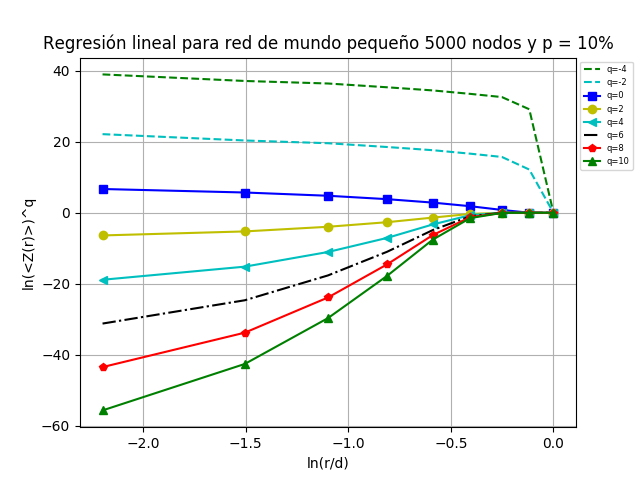
\includegraphics[scale=0.7]{Capitulo4Multifractalidad/imagenes/smallWorld5000p10_TqLnrBCsmallWorld5000p10.png}
    \caption{Regresión linea para red de mundo pequeño con 5000 nodos y $p=10\%$}
\end{figure}

A continuación, los exponentes de masa:


\begin{figure}[H]
    \centering
    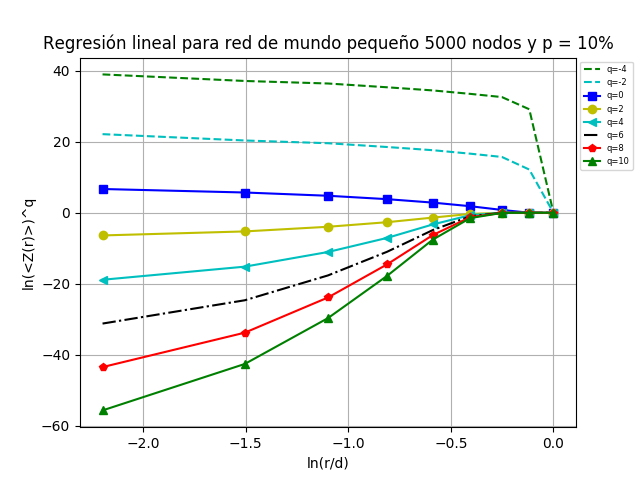
\includegraphics[scale=0.7]{Capitulo4Multifractalidad/imagenes/smallWorld5000p10_TqLnrBCsmallWorld5000p10.png}
    \caption{Exponentes de masa para red de mundo pequeño con 5000 nodos y $p=10\%$}
\end{figure}

Finalmente, la dimensión fractal generalizada


\begin{figure}[H]
    \centering
    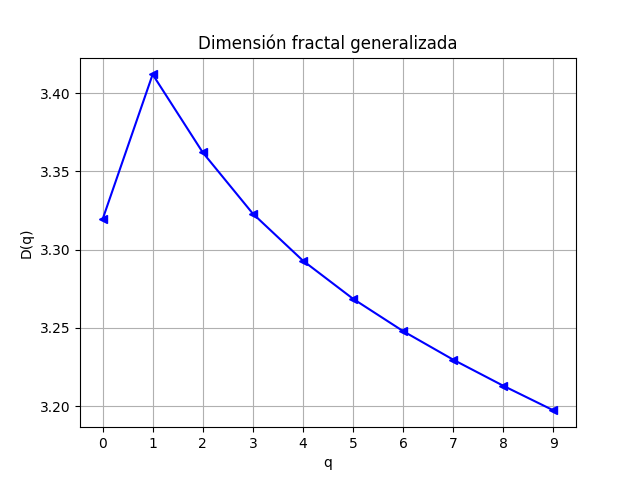
\includegraphics[scale=0.7]{Capitulo4Multifractalidad/imagenes/smallWorld5000p10_DqsmallWorld5000p10.png}
    \caption{Dimensión fractal generalizada para red de mundo pequeño con 5000 nodos y $p=10\%$}
\end{figure}

De acuerdo a los datos del articulo se encuentra:

\begin{table}[H]
    \centering
    \begin{tabular}{|c|c|c|}
        \hline
         \textbf{Dato}& \textbf{Valor obtenido} & \textbf{Valor articulo} \\
         \hline
         Dimensión fractal & 3.31 & 2.79 \\
         \hline
         Dimensión fractal generalizada & 3.41 & 2.8 \\
         \hline
         Dimensión de correlación & 3.36& 2.81 \\
         \hline
         Dimensión máxima & 3.41 & 2.81 \\
         \hline
         Dimensión mínima & 3.18 & 2.75 \\
         \hline
         Variación en la dimensión & 0.23 & 0.06 \\
         \hline
    \end{tabular}
    \caption{Datos obtenidos con el método Box Counting Fixed size comparando con datos del artículo de Wang\cite{Wang2012}}
\end{table}

Los resutlados varían ya que las redes del articulo y las utilizadas en estas pruebas son generadas, es decir que no son las mismas.

Se observa que la variación en la dimensión fractal es muy pequeña, por lo que se puede concluir que las redes libres de escala son monofractales, es decir que se pueden considerar como una sola estructura.

La dimensión fractal de esta red es 3.47



\subsubsection{Box Covering Compact}

Esta estrategia